\lab{Data Structures II: Trees}{Data Structures II}
\label{lab:Python_DataStructures2}

\objective{A \emph{Tree} is a linked list where each node in the list may refer to more than one other node. This structural flexibility makes trees more useful and efficient than regular linked lists in many applications. Many trees are most easily constructed recursively, so we begin with an overview of recursion. We then implement a recursively structured doubly linked Binary Search Tree. Finally, we compare the standard linked list, our Binary Search Tree, and an AVL tree to illustrate the relative strengths and weaknesses of each structure.}

\section*{Recursion} % ========================================================

A \emph{recursive} function is one that calls itself.
When the function is executed, it continues calling itself until it reaches a specified \emph{base case} where the solution to the problem is known.
The function then exits without calling itself again, and each previous function call is resolved.

As a simple example, consider the function that sums all positive integers from $1$ to some integer $n$.
This function may be represented recursively:
\[f(n) = \sum_{i=1}^ni = n + \sum_{i=1}^{n-1}i = n + f(n-1)\]
$f(n)$ may be calculated by recursively calculating $f(n-1)$, which calculates $f(n-2)$, and so on.
The recursion halts with the base case $f(1) = 1$.

\begin{lstlisting}
def recursive_sum(n):
	"""Calculate the sum of all positive integers in [1, n] recursively."""
    # Base Case: the sum of all positive integers in [1, 1] is 1.
	if n == 1:
		return 1

	# If the base case hasn't been reached, the function recurses by calling
    # itself on the next smallest integer. The result of that call, plus the
    # particular 'n' from this call, gives the result.
	else:
		return n + recursive_sum(n-1)
\end{lstlisting}

The computer calculates \li{recursive_sum(5)} with a sequence of function calls.

\begin{lstlisting}
# To find the recursive_sum(5), calculate recursive_sum(4).
# But to find recursive_sum(4), calculate recursive_sum(3).
# This continues until the base case is reached.

recursive_sum(5)		# return 5 + recursive_sum(4)
	recursive_sum(4)		# return 4 + recursive_sum(3)
		recursive_sum(3)		# return 3 + recursive_sum(2)
			recursive_sum(2)		# return 2 + recursive_sum(1)
				recursive_sum(1)		# Base case: return 1.
\end{lstlisting}

Substituting the values that resulted from each call unwinds the recursion.

\begin{lstlisting}
recursive_sum(5)		# return 5 + 10
	recursive_sum(4)		# return 4 + 6
		recursive_sum(3)		# return 3 + 3
			recursive_sum(2)		# return 2 + 1
				recursive_sum(1)		# Base case: return 1.
\end{lstlisting}

So \li{recursive_sum(5)} returns 15 (which is correct, since $1 + 2 + 3 + 4 + 5 = 15$).

Many problems that can be solved by iterative methods can also be solved (often more intuitively) with a recursive approach.
Consider the function $g:\mathbb{N}\rightarrow\mathbb{N}$ that calculates the $n^{th}$ Fibonacci number:
\[g(n) = g(n-1) + g(n-2),\quad g(0)=0,\quad g(1)=1\]
The mathematical function itself is defined recusively, so it makes sense for an implementation to use recursion.
Compare the following iterative method implementing $g$ to its recursive equivalent.

\begin{lstlisting}
def iterative_fib(n):
	"""Calculate the nth Fibonacci number iteratively."""
	fibonacci = []          # Initialize an empty list.
	fibonacci.append(0)		# Append 0 (the 0th Fibonacci number).
	fibonacci.append(1)		# Append 1 (the 1st Fibonacci number).
	for i in range(1, n):
		# Starting at the third entry, calculate the next number
		# by adding the last two entries in the list.
		fibonacci.append(fibonacci[-1] + fibonacci[-2])
	# When the entire list has been loaded, return the nth entry.
	return fibonacci[n]

def recursive_fib(n):
	"""Calculate the nth Fibonacci number recursively."""
	# The base cases are the first two Fibonacci numbers.
	if n == 0:				# Base case 1: the 0th Fibonacci number is 0.
		return 0
	elif n == 1:			# Base case 2: the 1st Fibonacci number is 1.
		return 1
	# If this call isn't a base case, the function recurses by calling
	# itself to calculate the previous two Fibonacci numbers.
	else:
		return recursive_fib(n-1) + recursive_fib(n-2)
\end{lstlisting}

This time, the sequence of function calls is slightly more complicated because \li{recursive_fib()} calls itself twice at each step.

\begin{lstlisting}
recursive_fib(5)		# The original call makes two additional calls:
	recursive_fib(4)		# this one...
		recursive_fib(3)
			recursive_fib(2)
				recursive_fib(1)		# Base case 2: return 1
				recursive_fib(0)		# Base case 1: return 0
			recursive_fib(1)		# Base case 2: return 1
		recursive_fib(2)
			recursive_fib(1)		# Base case 2: return 1
			recursive_fib(0)		# Base case 1: return 0
	recursive_fib(3)		# ...and this one.
		recursive_fib(2)
			recursive_fib(1)		# Base case 2: return 1
			recursive_fib(0)		# Base case 1: return 0
		recursive_fib(1)		# Base case 2: return 1
\end{lstlisting}

The sum of all of the base case results, from top to bottom, is $1 + 0 + 1 + 1 + 0 + 1 + 0 + 1 = 5$, so \li{recursive_fib(5)} returns 5 (correctly).
The key to recursion is understanding the base cases correctly and making correct recursive calls.

\begin{problem} % Simple recursion for linked lists traversal
The following code defines a simple class for singly linked lists.
\begin{lstlisting}
class SinglyLinkedListNode(object):
    """Simple singly linked list node."""
    def __init__(self, data):
        self.value, self.<<next>> = data, None

class SinglyLinkedList(object):
    """A very simple singly linked list with a head and a tail."""
    def __init__(self):
        self.head, self.tail = None, None
    def append(self, data):
        """Add a Node containing 'data' to the end of the list."""
        n = SinglyLinkedListNode(data)
        if self.head is None:
            self.head, self.tail = n, n
        else:
            self.tail.<<next>> = n
            self.tail = n
\end{lstlisting}
Rewrite the following iterative function for finding data in a linked list using recursion.
Use instances of the \li{SinglyLinkedList} class to test your function.
\begin{lstlisting}
def iterative_search(linkedlist, data):
    """Search 'linkedlist' iteratively for a node containing 'data'."""
	current = linkedlist.head
	while current is not None:
		if current.value == data:
			return current
		current = current.<<next>>
	raise ValueError(str(data) + " is not in the list.")
\end{lstlisting}
(Hint: define an inner function to perform the actual recursion.)
\label{prob:recursion}
\end{problem}

\begin{warn} % Iterative methods > Recursive methods, usually.
It is \textbf{not} usually better to rewrite an iterative method recursively.
In Python, a function may only call itself 999 times.
On the $1000^{th}$ call, a \li{RuntimeError} is raised to prevent a stack overflow.
Whether or not recursion is appropriate depends on the problem to be solved and the algorithm used to solve it.
\end{warn}

\section*{Trees} % ============================================================

A \emph{tree} data structure is a specialized linked list.
Trees are more difficult to build than standard linked lists, but they are almost always more efficient.
While the computational complexity of finding a node in a linked list is $O(n)$, a well-built, balanced tree will find a node with a complexity of $O(\log{n})$.
Some types of trees can be constructed quickly but take longer to retrieve data, while others take more time to build and less time to retrieve data.

The first node in a tree is called the \emph{root}.
The root node points to other nodes, called children.
Each child node in turn points to its children.
This continues on each branch until its end is reached.
A node with no children is called a \emph{leaf node}.

Mathematically, a tree is a directed graph with no cycles.
Therefore a linked lists as a graph qualifies as a tree, albeit a boring one.
The head node is the root node, and it has one child node.
That child node also has one child node, which in turn has one child.
The last node in the list is the only leaf node.

Other kinds of trees may be more complicated.

\section*{Binary Search Trees} % ==============================================

A \emph{binary search tree} (BST) data structure is a tree that allows each node to have up to two children, usually called \li{left} and \li{right}.
The left child of a node contains data that is less than its parent node's data.
The right child's data is greater.

The tree on the right in Figure \ref{fig:trees} is an example of a of binary search tree.
In practice, binary search tree nodes have attributes that keep track of their data, their children, and (in doubly linked trees) their parent.

\begin{figure}[H]
\begin{tikzpicture}[
    level 1/.style={sibling distance=2cm},
    level 2/.style={sibling distance=20mm}]

    \node [circle,draw] (4){4}
        child {node[draw, circle] (5) {5} edge from parent[draw=none]}
        child {node[circle,draw] (3) {3}edge from parent[draw=none]
        child{node[draw,circle](2){2}edge from parent[draw=none]}
        child{node[circle, draw](7){7}edge from parent[draw=none]}
        };
    \node [draw=none, node distance=.1cm] (4a)[above of=4]{}
        child {node[draw=none] (5a) {} edge from parent[draw=none]}
        child {node[draw=none] (3a) {}edge from parent[draw=none]
        child{node[draw=none](2a){}edge from parent[draw=none]}
        child{node[draw=none](7a){}edge from parent[draw=none]}
        };
    \node [draw=none, node distance=.1cm] (4b)[below of=4]{}
        child {node[draw=none] (5b) {} edge from parent[draw=none]}
        child {node[draw=none] (3b) {}edge from parent[draw=none]
        child{node[draw=none](2b){}edge from parent[draw=none]}
        child{node[draw=none](7b){}edge from parent[draw=none]}
        };
\foreach \s/\t in {4a/5a, 4a/3a, 5a/2a, 3a/7a}
    {\draw[->, >=stealth', shorten <=.23cm, shorten >=.1cm](\s)--(\t);}

\end{tikzpicture}
\qquad
\begin{tikzpicture}[
    auto,
    level 1/.style={sibling distance=2cm},
    level 2/.style={sibling distance=20mm}]

    \node [circle,draw] (5a){5}
        child {node[circle,draw] (2a) {2}edge from parent[draw=none]
            child { node[circle,draw] (1a) {1}edge from parent[draw=none]}
            child {node[draw = none] (invisble){} edge from parent[draw=none]}
        }
        child {node[circle,draw] (7a) {7}edge from parent[draw=none]
        child{node[circle, draw](6a){6}edge from parent[draw=none]}
        child{node[circle, draw](8a){8}edge from parent[draw=none]}
        };
    \node [draw=none, node distance=.1cm] (i5a)[above of=5a]{}
        child {node[draw=none] (i2a) {}edge from parent[draw=none]
            child { node[draw=none] (i1a) {}edge from parent[draw=none]}
            child {node[draw = none] (invisbleA){} edge from parent[draw=none]}
        }
        child {node[draw=none] (i7a) {}edge from parent[draw=none]
        child{node[draw=none](i6a){}edge from parent[draw=none]}
        child{node[draw=none](i8a){}edge from parent[draw=none]}
        };
\foreach \s/\t in {i5a/i2a, i5a/i7a}
    {\draw[->, >=stealth', shorten <=.23cm, shorten >=.1cm](\s)--(\t);}
\foreach \s/\t in {i2a/i1a, i7a/i6a, i7a/i8a}
    {\draw[->, >=stealth', shorten <=.27cm, shorten >=.1cm](\s)--(\t);}
\end{tikzpicture}
\caption{Both of these graphs are trees, but only the tree on the right is a binary search tree. How could the graph on the left be altered to make it a BST?}
\label{fig:trees}
\end{figure}

\begin{lstlisting}
class BSTNode(object):
    """A Node class for Binary Search Trees. Contains some data, a
    reference to the parent node, and references to two child nodes.
    """
    def __init__(self, data):
        """Construct a new node and set the data attribute. The other
        attributes will be set when the node is added to a tree.
        """
        self.value = data
        self.prev = None      # A reference to this node's parent node.
        self.left = None      # This node's value will be less than self.value
        self.right = None     # This node's value will be greater than self.value
\end{lstlisting}

The actual binary search tree class has an attribute pointing to its root.

\begin{lstlisting}
class BST(object):
    """Binary Search Tree data structure class.
    The 'root' attribute references the first node in the tree.
    """
    def __init__(self):
        """Initialize the root attribute."""
        self.root = None
\end{lstlisting}

\subsection*{find()} % --------------------------------------------------------

Finding a node in a binary search tree can be done recursively.
Starting at the root, check if the target data matches the current node.
If it does not, then if the data is less than the current node's value, search again on the left child.
If the data is greater, search on the right child.
Continue the process until the data is found or, if the data is not in the tree, an empty child is searched.

\begin{lstlisting}
class BST(object):
    # ...
    def find(self, data):
        """Return the node containing 'data'. If there is no such node
        in the tree, or if the tree is empty, raise a ValueError.
        """

        # Define a recursive function to traverse the tree.
        def _step(current):
            """Recursively step through the tree until the node containing
            'data' is found. If there is no such node, raise a Value Error.
            """
            if current is None:                     # Base case 1: dead end.
                raise ValueError(str(data) + " is not in the tree.")
            if data == current.value:               # Base case 2: data found!
                return current
            if data < current.value:                # Recursively search left.
                return _step(current.left)
            else:                                   # Recursively search right.
                return _step(current.right)

        # Start the recursion on the root of the tree.
        return _step(self.root)
\end{lstlisting}

\begin{info}
Conceptually, each node of a BST partitions the data of its subtree into two halves: the data that is less than the parent, and the data that is greater.
We will extend this concept to higher dimensions in the next lab.
\end{info}

\subsection*{insert()} % ------------------------------------------------------

To insert new data into a binary search tree, add a leaf node at the correct location.
First, find the node that should be the parent of the new node.
This parent node is found recursively, using a similar approach to the \li{find()} method.
Then the new node is added as the left or right child of the parent.
See Figure \ref{fig:BST.insertion}.

\begin{figure}[H] % BST.insert()
\begin{tikzpicture}[
    auto,
    level 1/.style={sibling distance=2cm},
    level 2/.style={sibling distance=20mm}]

    \node [circle,draw] (5a){5}
        child {node[circle,draw] (2a) {2}edge from parent[draw=none]
            child { node[circle,draw] (1a) {1}edge from parent[draw=none]}
            child {node[draw = none] (invisble){} edge from parent[draw=none]}
        }
        child {node[circle,draw] (7a) {7}edge from parent[draw=none]
        child{node[circle, draw](3a){3}edge from parent[draw=none]}
        child{node[circle, draw](8a){8}edge from parent[draw=none]}
        };
    \node [draw=none, node distance=.1cm] (i5a)[above of=5a]{}
        child {node[draw=none] (i2a) {}edge from parent[draw=none]
            child { node[draw=none] (i1a) {}edge from parent[draw=none]}
            child {node[draw = none] (invisbleA){} edge from parent[draw=none]}
        }
        child {node[draw=none] (i7a) {}edge from parent[draw=none]
        child{node[draw=none](i3a){}edge from parent[draw=none]}
        child{node[draw=none](i8a){}edge from parent[draw=none]}
        };
    \node [draw=none, node distance=.1cm] (i5b)[below of=5a]{}
        child {node[draw=none] (i2b) {}edge from parent[draw=none]
            child { node[draw=none] (i1b) {}edge from parent[draw=none]}
            child {node[draw = none] (invisbleB){} edge from parent[draw=none]}
        }
        child {node[draw=none] (i7b) {}edge from parent[draw=none]
        child{node[draw=none](i3b){}edge from parent[draw=none]}
        child{node[draw=none](i8b){}edge from parent[draw=none]}
        };
\node [draw=none, black!20!blue, node distance=1.5cm](root)[above right of=5a]{root};
\draw[black!20!blue, ->, >=stealth', shorten >= .1cm](root)--(5a);
\foreach \s/\t in {i5a/i2a, i2b/i5b, i5a/i7a, i7b/i5b}
    {\draw[->, >=stealth', shorten <=.23cm, shorten >=.1cm](\s)--(\t);}
\foreach \s/\t in {i2a/i1a, i1b/i2b, i7a/i8a, i8b/i7b}
    {\draw[->, >=stealth', shorten <=.27cm, shorten >=.1cm](\s)--(\t);}
\end{tikzpicture}
\qquad
\begin{tikzpicture}[
    auto,
    level 1/.style={sibling distance=2cm},
    level 2/.style={sibling distance=20mm}]

    \node [circle,draw] (5a){5}
        child {node[circle,draw] (2a) {2}edge from parent[draw=none]
            child { node[circle,draw] (1a) {1}edge from parent[draw=none]}
            child {node[draw = none] (invisble){} edge from parent[draw=none]}
        }
        child {node[circle,draw] (7a) {7}edge from parent[draw=none]
        child{node[circle, draw](3a){3}edge from parent[draw=none]}
        child{node[circle, draw](8a){8}edge from parent[draw=none]}
        };
    \node [draw=none, node distance=.1cm] (i5a)[above of=5a]{}
        child {node[draw=none] (i2a) {}edge from parent[draw=none]
            child { node[draw=none] (i1a) {}edge from parent[draw=none]}
            child {node[draw = none] (invisbleA){} edge from parent[draw=none]}
        }
        child {node[draw=none] (i7a) {}edge from parent[draw=none]
        child{node[draw=none](i3a){}edge from parent[draw=none]}
        child{node[draw=none](i8a){}edge from parent[draw=none]}
        };
    \node [draw=none, node distance=.1cm] (i5b)[below of=5a]{}
        child {node[draw=none] (i2b) {}edge from parent[draw=none]
            child { node[draw=none] (i1b) {}edge from parent[draw=none]}
            child {node[draw = none] (invisbleB){} edge from parent[draw=none]}
        }
        child {node[draw=none] (i7b) {}edge from parent[draw=none]
        child{node[draw=none](i3b){}edge from parent[draw=none]}
        child{node[draw=none](i8b){}edge from parent[draw=none]}
        };
\node [draw=none, black!20!blue, node distance=1.5cm](root)[above right of=5a]{root};
\draw[black!20!blue, ->, >=stealth', shorten >= .1cm](root)--(5a);
\node [draw=none, black!20!blue, node distance=1.5cm](parent)[above left of=2a]{parent};
\draw[black!20!blue, ->, >=stealth', shorten >= .1cm](parent)--(2a);
\foreach \s/\t in {i5a/i2a, i2b/i5b, i5a/i7a, i7b/i5b}
    {\draw[->, >=stealth', shorten <=.23cm, shorten >=.1cm](\s)--(\t);}
\foreach \s/\t in {i2a/i1a, i1b/i2b, i2a/i3a, i3b/i2b, i7a/i8a, i8b/i7b}
    {\draw[->, >=stealth', shorten <=.27cm, shorten >=.1cm](\s)--(\t);}
\foreach \s/\t in {i2a/i3a, i3b/i2b}
    {\draw[red, ->, >=stealth', shorten <=.27cm, shorten >=.1cm](\s)--(\t);}
\end{tikzpicture}
\caption{To insert a node containing 3 to the BST on the left, start at the root and recurse down the tree to find the node that should be 3's parent. Connect that parent to the child, then the child to its new parent.}
\label{fig:BST.insertion}
\end{figure}

\begin{problem} % BST.insert()
Implement the \li{insert()} method in the \li{BST} class.
%
\begin{enumerate}
\item Find the parent of the new node.
Consider writing a recursive method, similar to \li{find()}, to do this.
Determine whether the new node will be the parent's left or right child, then double-link the parent and the new child.
\item Do not allow for duplicates in the tree. Raise a \li{ValueError} if there is already a node in the tree containing the input data.
\end{enumerate}

Be sure to consider the special case of inserting to an empty tree.
To test your tree, use (but do not modify) the provided \li{BST.__str__()} method.
\end{problem}

\subsection*{remove()} % ------------------------------------------------------

Deleting nodes from a binary search tree is more difficult than finding or inserting.
Insertion always creates a new leaf node, but removal may delete any kind of node.
This leads to several different cases to consider.

\subsubsection*{Removing a Leaf Node} % - - - - - - - - - - - - - - - - - - - -

In Python, an object is automatically deleted if there are no references to it.
Call the node to be removed the \emph{target node}, and suppose it has no children.
To remove the target, find the target's parent, then delete the parent's reference to the target.
Then there are no references to the target, so the target node is deleted.
Since the target is a leaf node, removing it does not affect the rest of the tree structure.

\subsubsection*{Removing a Node with One Child} % - - - - - - - - - - - - - - -

If the target node has one or more children, be careful not to delete the children when the target is removed.
Simply removing the target as if it were a leaf node would delete the entire subtree originating from the target.

To avoid deleting all of the target's descendents, point the target's parent to an appropriate successor.
If the target has only one child, then that child is the successor.
Connect the target's parent to the successor, and double-link by setting the successor's parent to be the target node's parent.
Then, since the target has no references pointing to it, it is deleted.
The target's successor, however, is pointed to by the target's parent, and so it remains in the tree.
% TODO: Perhaps a figure for this one, as it is the hardest one to implement.

\subsubsection*{Removing a Node with Two Children} % - - - - - - - - - - - - -

Removal is more complicated if the target node has two children.
To delete this kind of node, first find its immediate in-order successor.
This successor is the node with the smallest value that is larger than the target's value.
It may be found by moving to the right child of the target (so that it's value is greater than the target's value), and then to the left for as long as possible (so that it has the smallest such value).
Note that because of how the successor is chosen, any in-order successor can only have at most one child.

Once the successor is found, the target and its successor must switch places in the graph, and then the target must be removed.
This can be done by simply switching the values for the target and its successor.
Then the node with the target data has at most one child, and may be deleted accordingly.
If the successor was chosen appropriately, then the binary search tree structure and ordering will be maintained once the deletion is finished.

The easiest way to implement this is to use recursion.
First, because the successor has at most one child, remove the successor node recursively by calling \li{remove()} on the successor's value.
Then set the data stored in the target node as the successor's value.
See Figure \ref{fig:BST.remove_twoChild}.

\begin{figure} % BST.remove() for removing a node with two children.
\begin{tikzpicture}[
    auto,
    level 1/.style={sibling distance=2cm},
    level 2/.style={sibling distance=20mm}]

    \node [circle,draw] (5){5}
        child {node[circle,draw] (2) {2}edge from parent[draw=none]
            child { node[circle,draw] (1) {1}edge from parent[draw=none]
            child{node[draw=none](invisible){} edge from parent[draw=none]}
            child{node[draw,circle](3){3} edge from parent[draw=none]}
       }
            child {node[draw, circle] (4){4} edge from parent[draw=none]}
        }
    child {node[circle,draw] (9a) {9}edge from parent[draw=none]
        child{node[draw=none](8){}edge from parent[draw=none]}
        };
    \node [draw=none, node distance=.1cm] (5a)[above of=5]{}
        child {node[draw=none] (2a) {}edge from parent[draw=none]
            child { node[draw=none] (1a) {}edge from parent[draw=none]
            child{node[draw=none](invisibleA){} edge from parent[draw=none]}
            child{node[draw=none](3a){} edge from parent[draw=none]}
        }
            child {node[draw = none] (4a){} edge from parent[draw=none]}
        }
        child {node[draw=none] (9a) {}edge from parent[draw=none]
        child{node[draw=none](8a){}edge from parent[draw=none]}
        };

    \node [draw=none, node distance=.1cm] (5b)[below of=5]{}
        child {node[draw=none] (2b) {}edge from parent[draw=none]
            child { node[draw=none] (1b) {}edge from parent[draw=none]
            child{node[draw=none](invisibleB){} edge from parent[draw=none]}
            child{node[draw=none](3b){} edge from parent[draw=none]}
        }
            child {node[draw = none] (4b){} edge from parent[draw=none]}
        }
        child {node[draw=none] (9b) {}edge from parent[draw=none]
        child{node[draw=none](8b){}edge from parent[draw=none]}
        };
\node [draw=none, black!20!blue, node distance=2cm](target)[left of=2a]{target};
\draw[black!20!blue, ->, >=stealth', shorten >= .2cm](target)--(2a);
\node [draw=none, black!20!blue, node distance=2cm](successor)[right of=3a]{successor};
\draw[black!20!blue, ->, >=stealth', shorten >= .2cm](successor)--(3a);
\foreach \s/\t in {2a/1a, 1b/2b, 2a/4a, 4b/2b, 5a/2a, 2b/5b, 5a/9a, 9b/5b, 4a/3a, 3b/4b}
    {\draw[->, >=stealth', shorten <=.23cm, shorten >=.1cm](\s)--(\t);}
\end{tikzpicture}
\qquad
\begin{tikzpicture}[
    auto,
    level 1/.style={sibling distance=2cm},
    level 2/.style={sibling distance=20mm}]

    \node [circle,draw] (5){5}
        child {node[circle,draw] (2) {3}edge from parent[draw=none]
            child { node[circle,draw] (1) {1}edge from parent[draw=none]
            child{node[draw=none](invisible){} edge from parent[draw=none]}
            child{node[draw,circle](3){2} edge from parent[draw=none]}
       }
            child {node[draw, circle] (4){4} edge from parent[draw=none]}
        }
    child {node[circle,draw] (9a) {9}edge from parent[draw=none]
        child{node[draw=none](8){}edge from parent[draw=none]}
        };
    \node [draw=none, node distance=.1cm] (5a)[above of=5]{}
        child {node[draw=none] (2a) {}edge from parent[draw=none]
            child { node[draw=none] (1a) {}edge from parent[draw=none]
            child{node[draw=none](invisibleA){} edge from parent[draw=none]}
            child{node[draw=none](3a){} edge from parent[draw=none]}
        }
            child {node[draw = none] (4a){} edge from parent[draw=none]}
        }
        child {node[draw=none] (9a) {}edge from parent[draw=none]
        child{node[draw=none](8a){}edge from parent[draw=none]}
        };

    \node [draw=none, node distance=.1cm] (5b)[below of=5]{}
        child {node[draw=none] (2b) {}edge from parent[draw=none]
            child { node[draw=none] (1b) {}edge from parent[draw=none]
            child{node[draw=none](invisibleB){} edge from parent[draw=none]}
            child{node[draw=none](3b){} edge from parent[draw=none]}
        }
            child {node[draw = none] (4b){} edge from parent[draw=none]}
        }
        child {node[draw=none] (9b) {}edge from parent[draw=none]
        child{node[draw=none](8b){}edge from parent[draw=none]}
        };
\node [draw=none, black!20!blue, node distance=2cm](target)[left of=2a]{target};
\draw[black!20!blue, ->, >=stealth', shorten >= .2cm](target)--(2a);
\node [draw=none, black!20!blue, node distance=2cm](successor)[right of=3a]{successor};
\draw[black!20!blue, ->, >=stealth', shorten >= .2cm](successor)--(3a);
\foreach \s/\t in {2a/1a, 1b/2b, 2a/4a, 4b/2b, 5a/2a, 2b/5b, 5a/9a, 9b/5b}
    {\draw[->, >=stealth', shorten <=.23cm, shorten >=.1cm](\s)--(\t);}
\end{tikzpicture}
\caption{To remove the node containing 2 from the top left BST, locate the target and its in-order successor. Delete the successor, recording its value. Finally, replace the data in the target with the data that was in the successor.}
\label{fig:BST.remove_twoChild}
\end{figure}

\subsubsection*{Removing the Root Node} % - - - - - - - - - - - - - - - - - - -

In each of the above cases, we must also consider the subcase where the target is the root node.
If the root has no children, resetting the root or calling the constructor will do.
If the root has one child, that child becomes the new root of the tree.
If the root has two children, the successor becomes the new root of the tree.

\begin{problem} % BST.remove()
Implement the \li{remove()} method in the \li{BST} class.
If the tree is empty, or if the target node is not in the tree, raise a \li{ValueError}.
Test your solutions thoroughly, accounting for all possible cases:
\begin{enumerate}
\item The tree is empty (\li{ValueError}).
\item The target is not in the tree (\li{ValueError}).
\item The target is the root node:
	\begin{enumerate}
	\item the root is a leaf node, hence the only node in the tree.
	\item the root has one child.
	\item the root has two children.
	\end{enumerate}
\item The target is in the tree but is not the root:
	\begin{enumerate}
	\item the target is a leaf node.
	\item the target has one child.
	\item the target has two children.
	\end{enumerate}
\end{enumerate}
(Hints: \textbf{Before coding anything}, outline the entire function with comments and \li{if}-\li{else} blocks.
Use the \li{find()} method wherever appropriate.)
\end{problem}

\section*{AVL Trees} % ========================================================

Binary search trees are a good way of organizing data so that it is quickly accessible.
However, pathologies may arise when certain data sets are stored using a basic binary serch tree.
This is best demonstrated by inserting ordered data into a binary search tree.
Since the data is already ordered, each node will only have one child, and the result is essentially a linked list.

\begin{lstlisting}
# Sequentially adding ordered integers destroys the efficiency of a BST.
>>> unbalanced_tree = BST()
>>> for i in range(10):
...     unbalanced_tree.insert(i)
...
# The tree is perfectly flat, so it loses its search efficiency.
>>> print(unbalanced_tree)
[0]
[1]
[2]
[3]
[4]
[5]
[6]
[7]
[8]
[9]
\end{lstlisting}

Problems also arise when one branch of the tree becomes much longer than the others, leading to longer search times.

An \emph{AVL tree} (named after Georgy Adelson-Velsky and Evgenii Landis) is a tree that prevents any one branch from getting longer than the others.
It accomplishes this by recursively ``balancing'' the branches as nodes are added.
See Figure \ref{fig:avl_balance}.
The AVL's balancing algorithm is beyond the scope of this project, but details and exercises on the algorithm can be found in Chapter 2 of the Volume II text.

\begin{figure}[H] % AVL Tree
\begin{tikzpicture}[
    auto,
    level 1/.style={sibling distance=2cm},
    level 2/.style={sibling distance=20mm}]

    \node [circle,draw] (4){4}
    child{node[draw, circle](2){2}edge from parent[draw=none]
        child{node[draw, circle](1){1}edge from parent[draw=none]}
        child{node[draw, circle](3){3}edge from parent[draw=none]}
    }
    child{node[draw,circle](5){5}edge from parent[draw=none]
        child{node[draw=none](invisible){}edge from parent[draw=none]}
        child{node[draw, circle](6){6}edge from parent[draw=none]}
    };

    \node [draw=none, node distance=.1cm] (4a)[above of=4]{}
    child{node[draw=none](2a){}edge from parent[draw=none]
        child{node[draw=none](1a){}edge from parent[draw=none]}
        child{node[draw=none](3a){}edge from parent[draw=none]}
    }
    child{node[draw=none](5a){}edge from parent[draw=none]
        child{node[draw=none](invisibleA){}edge from parent[draw=none]}
        child{node[draw=none](6a){}edge from parent[draw=none]}
    };

    \node [draw=none, node distance=.1cm] (4b)[below of=4]{}
    child{node[draw=none](2b){}edge from parent[draw=none]
        child{node[draw=none](1b){}edge from parent[draw=none]}
        child{node[draw=none](3b){}edge from parent[draw=none]}
    }
    child{node[draw=none](5b){}edge from parent[draw=none]
        child{node[draw=none](invisibleB){}edge from parent[draw=none]}
        child{node[draw=none](6b){}edge from parent[draw=none]}
    };

\foreach \s/\t in {4a/2a, 2a/1a, 2a/3a, 4a/5a, 5a/6a}
    {\draw[->, >=stealth', shorten <=.23cm, shorten >=.1cm](\s)--(\t);}
\node [draw=none, black!20!blue, node distance=1.5cm](root)[above right of=4a]{root};
\draw[black!20!blue, ->, >=stealth', shorten >= .1cm](root)--(4);

\end{tikzpicture}
\caption{The balanced AVL tree resulting from inserting 1, 2, 3, 4, 5, and 6, in that order. After each insertion the tree rebalances if necessary.}
\label{fig:avl_balance}
\end{figure}

\newpage

\begin{lstlisting}
>>> balanced_tree = AVL()
>>> for i in range(10):
...     balanced_tree.insert(i)
...
# The AVL tree is balanced, so it retains (and optimizes) its search efficiency.
>>> print(balanced_tree)
[3]
[1, 7]
[0, 2, 5, 8]
[4, 6, 9]
\end{lstlisting}

% Problem 4: compare build and search speeds.
% TODO (?): Instead of a file to read from, have them generate random numbers.
%   Reading data from a file is an over-complication (abolish English.txt).
\begin{problem}
Write a function to compare the build and search speeds of the data structures we have implemented so far.

Accept a file name to read from.
Read the file, adding the contents of each line to a list of data.
For various values of $n$, repeat the following:
%
\begin{enumerate}
\item Get a subset of $n$ items from the data set.
\item Time (separately) how long it takes to load a new \li{SinglyLinkedList}, a \li{BST}, and an \li{AVL} with the $n$ items.
\item Choose 5 \textbf{random} items from the subset, and time how long it takes to find all 5 items in each data structure.
To avoid exceeding the maximum recursion depth, use the provided \li{iterative_search()} function from Problem \ref{prob:recursion} to search the \li{SinglyLinkedList}.
\end{enumerate}

Report your findings in a single figure with two subplots: one for build times, and one for search times.
Use log scales where appropriate.
\begin{comment} % TODO: Decide whether or not to show them these plots.
Your figure should resemble the following plots, though your results may be less smooth.
%
\begin{figure}[H] % Solution to problem 4.
    \centering
    \begin{subfigure}[b]{.5\textwidth}
        \centering
        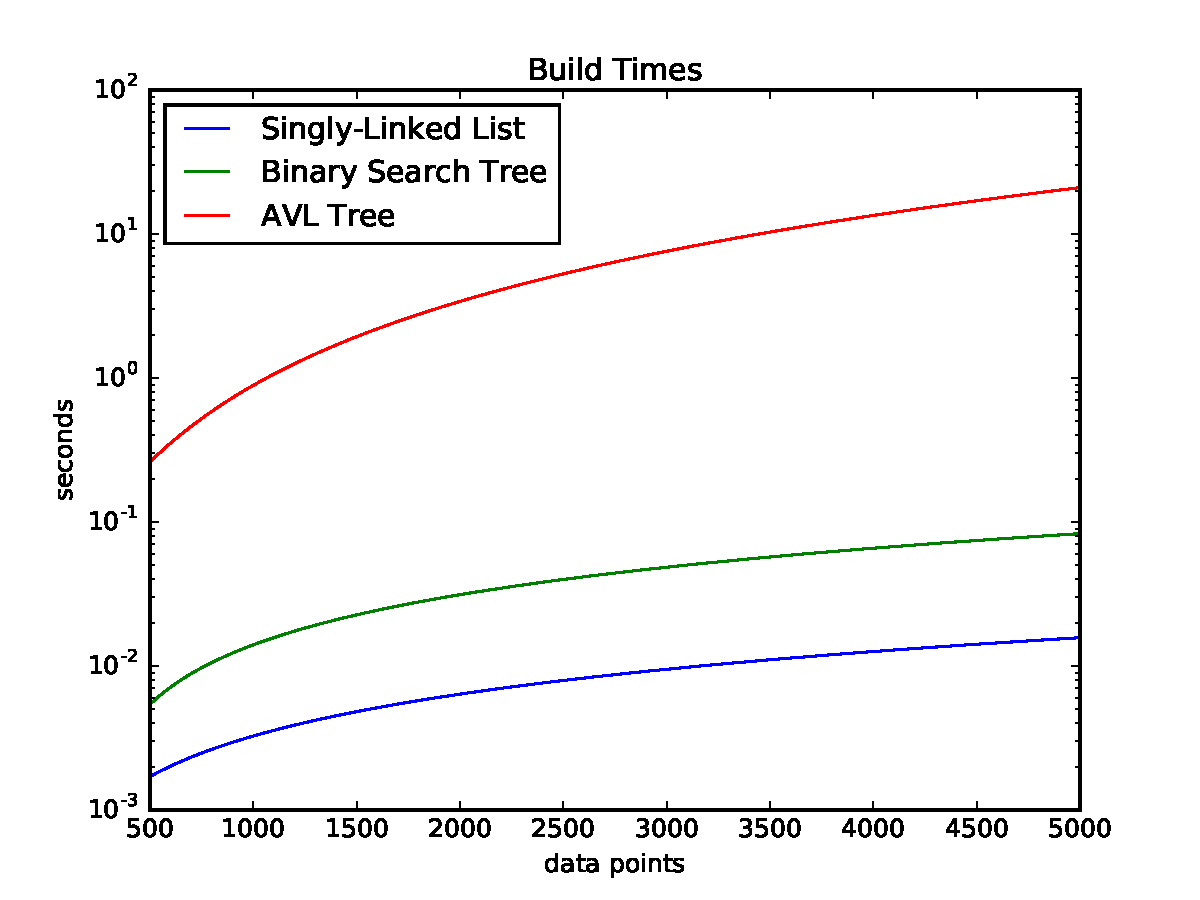
\includegraphics[width=\textwidth]{BuildTimes.pdf}
    \end{subfigure}%
    \begin{subfigure}[b]{.5\textwidth}
        \centering
        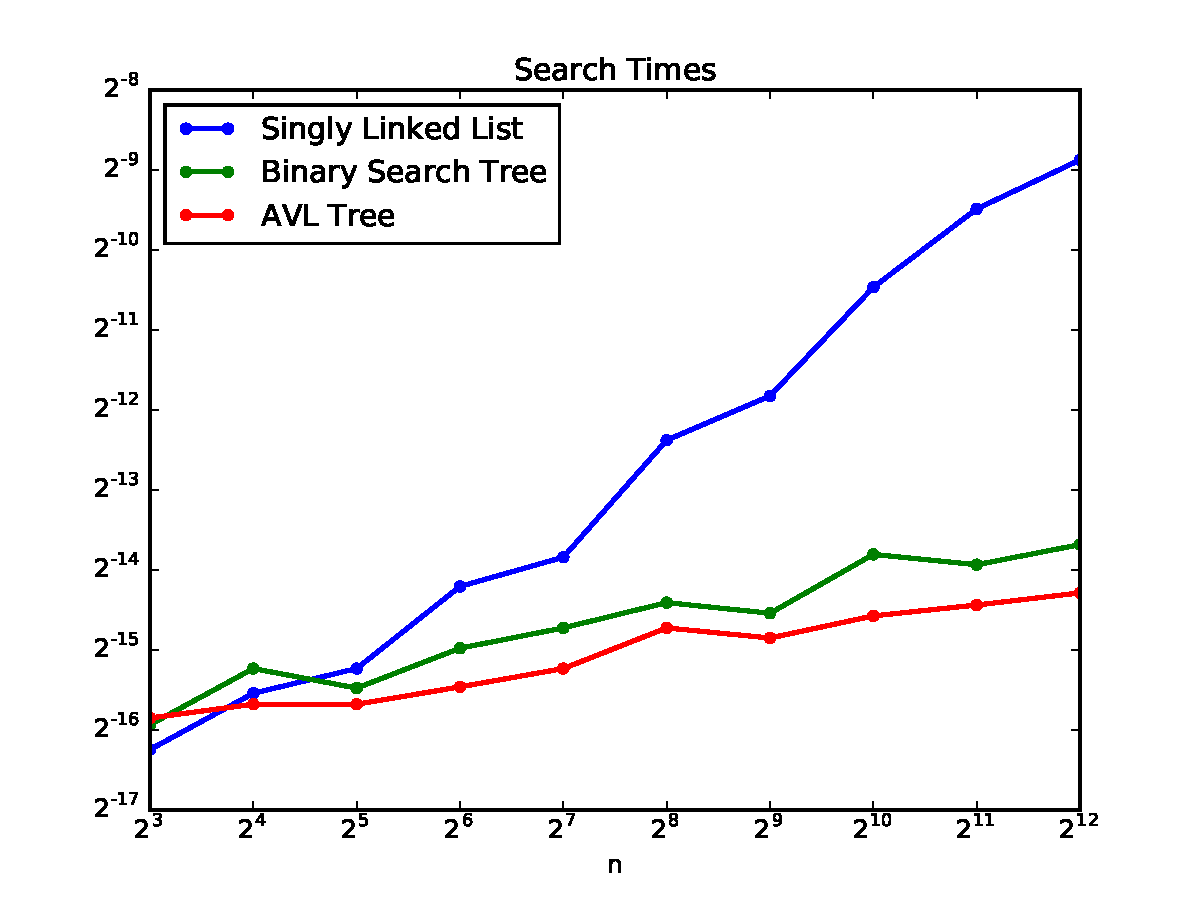
\includegraphics[width=\textwidth]{SearchTimes.pdf}
    \end{subfigure}
    % \caption{The \li{SinglyLinkedList} has the fastest build times, but the \li{AVL} has the fastest search times. How would the graphs be different if the data had been sorted to begin with?}
\end{figure}
\end{comment}
\end{problem}

\section*{Conclusion} % =======================================================

Every data structure has advantages and disadvantages.
Recognizing when an application may take advantage of a certain structure, especially when that structure is more complicated than a Python list or set, is an important skill.
Choosing structures wisely often results in huge speedups and easier data maintenance.

\newpage

\section*{Additional Material} % ==============================================

\subsection*{Improvements to the BST} % ---------------------------------------
The following are ideas for improving the \li{BST} class.

\begin{enumerate}
\item Modify the constructor so that it accepts an optional argument . . .
\item Add an attribute that keeps track of the number of items in the tree.
Use this attribute to implement the \li{__len__()} magic method.
\item Add a method for translating the \li{BST} into a regular Python list using a depth-first search.
\end{enumerate}

\subsection*{Other Trees} % ---------------------------------------------------

There are many variations on the Binary Search Tree, each with its own advantages and disadvantages.
Consider writing classes for the following structures.
%
\begin{enumerate}
\item A \href{https://en.wikipedia.org/wiki/B-tree}{\emph{B-Tree}} is a tree whose nodes can contain more than one piece of data.
\item The nodes of a \href{https://en.wikipedia.org/wiki/Red%E2%80%93black_tree}{\emph{Red-Black Tree}} are labeled either red or black.
\item A \href{https://en.wikipedia.org/wiki/Splay_tree}{\emph{Splay Tree}} is interesting.
\end{enumerate}

